% ============================================================================
% DRAFT v2 -- Section 5: Where the leverage actually is
% Numbers from fusion_policy/fusion_summary.json (E2), policy_select/ (E3),
% pseudo_select/ (E9, pending).
% ============================================================================

\section{Results: Where the Leverage Is --- the Inference-Time Scoring Policy}
\label{sec:leverage}

Section~\ref{sec:diagnosis} established that the design axis the pipeline
searches---the backbone---does not measurably move accuracy, while the search
signal used to choose within it is unstable. That raises an obvious question:
which design choices \emph{do} move accuracy? This section shows that the way
per-pixel discrepancies are combined into an image-level score---a choice that
requires no additional training to revisit---is worth an order of magnitude more
than the architecture.

\subsection{The Scoring Policy as a Design Axis}
\label{subsec:policy_space}

With a trained detector the anomaly score of an image is formed in two steps
(Section~\ref{subsec:rd_detection}): the discrepancy maps $m_1, m_2, m_3$ of the
three teacher scales are combined by non-negative weights, and the resulting map
is reduced to a scalar. The published pipeline fixes both choices implicitly:
uniform weights, and the arithmetic mean over all pixels.

Neither is forced by the method. We therefore treat the pair
$(\mathbf{w}, \rho)$ as a \emph{scoring policy}, with
$\mathbf{w}$ on the probability simplex over three scales and
$\rho \in \{\text{mean}, \text{top-}k, \text{max}\}$, where top-$k$ averages the
$k$ highest-scoring pixels with $k = 1\%$ of the map. We evaluate 82 policies:
the 66-point simplex grid at step $0.1$ crossed with top-$k$ pooling, plus 9
single-scale policies (\texttt{s1}, \texttt{s2}, \texttt{s3} $\times$ mean, top-$k$,
max), 3 policies that sum the three maps without weights, and 4 that normalise each
map before combining ($66+9+3+4 = 82$). The exact enumeration, with every
$(\mathbf{w},\rho)$ pair keyed by name, is released in
\texttt{fusion\_policy/fusion\_summary.json}.

A second and larger policy set is used in
Section~\ref{subsec:pseudo_results}, where the search over policies has to be
richer because the criterion rather than the pooling is under test: the finer
simplex grid at step $0.2$ is paired with all three reductions, and the coarser
step-$0.1$ grid is paired with top-$k$ pooling, together with the three canonical
uniform variants, giving $66 + 21 + 21 + 3 = 111$ policies. The two sets are not
interchangeable, and the numbers below are quoted per set; where they are compared
directly, Table~\ref{tab:ksweep} says so.

An important property of this axis is that a fixed grid of it can be evaluated
without retraining: changing $(\mathbf{w},\rho)$ requires no new parameters and no
extra inference, since the discrepancy maps are already computed and pooling is a
reduction over them, so every policy in the grid is evaluated on the \emph{same}
trained model. The simplex is continuous, so no finite grid can be exhaustive;
what we evaluate is a fixed grid of the size stated above, and the sensitivity
sweep of Section~\ref{subsec:policy_results} is what establishes that the grid is
fine enough for the conclusion. This is a practical convenience for deployment ---
the policy can be
re-tuned on an existing detector without repeating the training run --- and it is
what makes the grid evaluation below affordable.

It is worth being explicit that this does not diminish the role of training, and
we do not present the two axes as competing. Establishing that the architecture
axis is inert (Section~\ref{sec:diagnosis}) required retraining hundreds of
detectors, and we regard that expense as the necessary price of a defensible
claim. The axes are complementary: training determines what a model can
represent, and the scoring policy determines how much of that is read out.

\subsection{Exhaustive Evaluation on a Fixed Model}
\label{subsec:policy_results}

We train one detector per MVTec-AD category with the manuscript's protocol
(EfficientNet-B0 student, 500 epochs, batch size 64, seed 42, ResNet-18 teacher),
then evaluate all 82 policies on the frozen model. Table~\ref{tab:fusion} reports
the result.

\begin{table}[t]
\centering
\caption{Scoring policies evaluated on one frozen detector per category
(15 categories, 82 policies). ``Worst category'' is the lowest per-category
AUROC, i.e.\ the failure mode that matters in deployment. The default is the
policy the published pipeline uses. The per-category oracle \emph{reads the test
labels} to pick the best policy for each category and is an upper bound, not an
achievable result; every other row is label-free.}
\label{tab:fusion}
\resizebox{\columnwidth}{!}{%
\begin{tabular}{lrrr}
\toprule
Policy & Mean AUROC (\%) & Worst category (\%) & Extra retraining \\
\midrule
\texttt{mean}, uniform weights (default) & 82.80 & \textbf{42.22} & --- \\
\texttt{max}, uniform weights            & 86.84 & --- & none \\
\texttt{top-}k, uniform weights          & 90.21 & 78.37 & none \\
best single policy over the grid (\texttt{w0.3\_0.6\_0.1}, top-$k$; picked on
test, so also an oracle) & \textbf{90.60} & --- & none \\
\midrule
per-category oracle over 82 policies (uses labels)     & \textbf{93.72} & 84.67 & none \\
\bottomrule
\end{tabular}}

\end{table}

Switching the pooling from the arithmetic mean to top-$k$ raises mean AUROC from
$82.80\%$ to $90.21\%$, a gain of $7.42$ points, with no change to the model.
(Throughout this section the deltas are computed on the unrounded values and
rounded only for display, so a delta may differ by $0.01$ from the subtraction of
the two printed figures --- here $90.2075 - 82.7896 = 7.4179$.)
Scale weighting adds much less: the best weighted policy reaches $90.60\%$, only
$0.39$ points above the uniform top-$k$. Every one of the eight highest-scoring
policies uses top-$k$ pooling, and all of the improvement therefore comes from
the reduction step rather than from the scale weights. Choosing the policy
per category raises the mean further, to $93.72\%$---$10.92$ points above the
default, and again without retraining anything.

The pooling effect is not an artefact of one training run. Repeating the
comparison with two further seeds (43 and 44) gives $+8.07$ and $+7.78$ points
against $+7.42$ for the seed reported here; the per-seed estimates span
$0.65$ points. Aggregating the two later seeds alone gives policy means of
$82.36\%$ for the default and $90.28\%$ for top-$k$ ($+7.92$ points, seeds
$43$--$44$). We quote the per-seed estimates and that within-script aggregate
rather than one summary number, because seed~42's models enter the reported table
through a different evaluation script than the later two do
(Table~\ref{tab:ksweep}): averaging across the two scripts would average two
implementations of the same statistic, which we decline to do, so we do not quote a
single three-seed mean for this quantity.
Throughout, the seed reported in full is seed~42, on which the default and top-$k$
read $82.80\%$ and $90.21\%$ ($+7.42$); the headline we carry into the abstract
and conclusion is the conservative $+7.5$ points, the mean on the label-free
$70/30$ split of Section~\ref{subsec:pseudo_results}. Every quantity we can
measure for this effect therefore lies between $+7.4$ and $+8.1$ points, and we
quote the smallest of them as the headline.

\runinhead{The effect is not a hyper-parameter artefact.}
The comparison fixes $k = 1\%$ of the map, so it is fair to ask whether the gain
is an artefact of that choice. Sweeping $k$ over two orders of magnitude
(Table~\ref{tab:ksweep} and Figure~\ref{fig:ksweep}) traces a broad plateau rather than a spike: mean AUROC
rises from $86.74\%$ at $k = 1$ pixel to a maximum of $91.08\%$ at $k = 5\%$, and
stays above $89.6\%$ for every $k$ between $0.5\%$ and $20\%$. The default of
$1\%$ sits inside the plateau, not on its edge, and any value in that range
recovers $7$ to $8.4$ points. The worst-category statistic peaks earlier, at
$k = 2\%$ ($79.24\%$), so $k$ between $1\%$ and $2\%$ is the best compromise
between average accuracy and worst-case behaviour.

\begin{figure}[t]
\centering
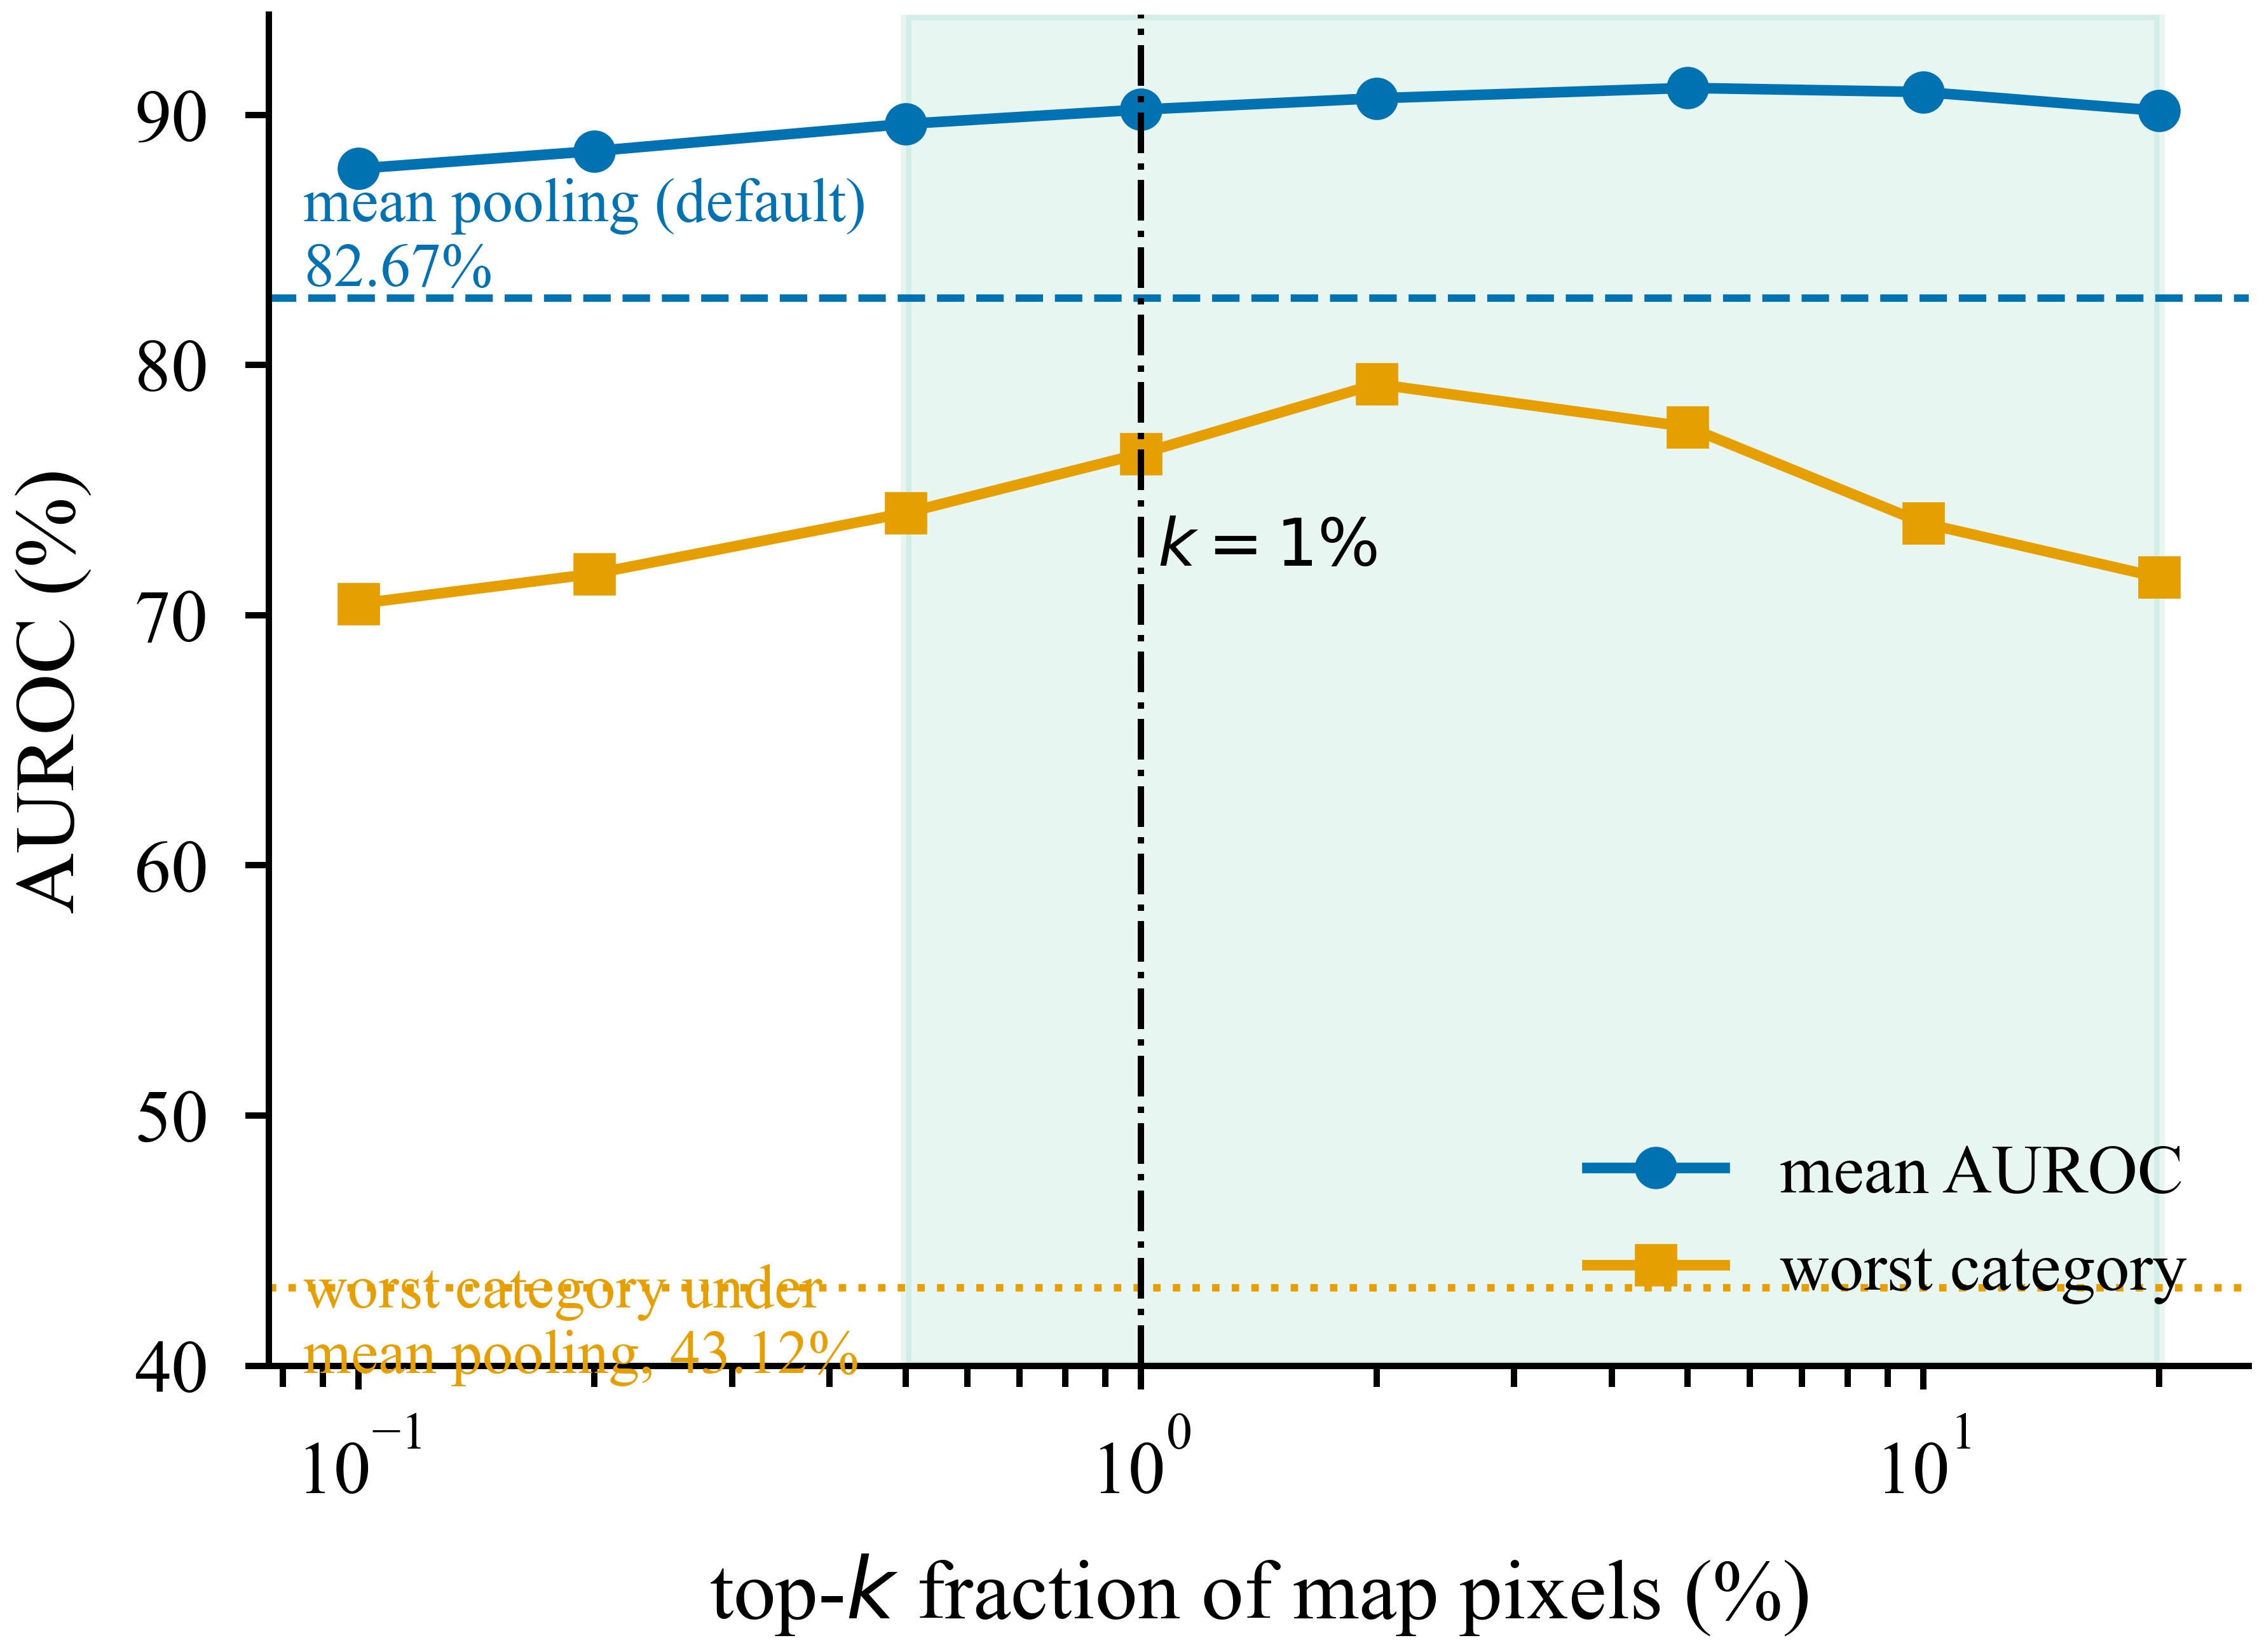
\includegraphics[width=\linewidth]{figures_v2/fig5_topk_sensitivity.png}
\caption{Sensitivity of the pooling gain to the top-$k$ fraction. The effect is a
broad plateau, not a spike: every $k$ between $0.5\%$ and $20\%$ recovers $7$ to
$8.4$ points of mean AUROC relative to mean pooling, and the published choice of
$k = 1\%$ lies inside the plateau rather than on its edge. The worst category peaks
earlier, at $k = 2\%$.}
\label{fig:ksweep}
\end{figure}

\begin{table}[t]
\centering
\caption{Sensitivity of the pooling gain to the top-$k$ fraction, uniform weights,
15 categories, computed by a second evaluation script on the same seed-42 trained
models. Every row in this table shares those maps, so the comparison is internally
exact. The two scripts \emph{disagree per category} even though their 15-category
means agree: for the identical policy (\texttt{sum\_topk} in the first script,
\texttt{uniform|topk\_0.01} in the second) the two read $90.21\%$ both, but their
per-category values differ by a mean absolute $0.74$ points and up to $2.49$
points (\texttt{tile}: $85.79$ vs $88.28$), and the worst-category statistic ---
the stated rationale for the $k$ range recommended below --- differs by $1.91$
points (\texttt{pill}: $78.37$ vs $76.46$). The default policy reads $82.67\%$
here against $82.80\%$ in Table~\ref{tab:fusion}, a $0.13$-point aggregate
difference that is the same level at which the two implementations agree on this
pipeline. We keep both scripts in the release and quote the range rather than
select one, and we flag that the per-category and worst-category numbers in this
section should be read as implementation-dependent to about two points. Two more
such pairs, for completeness: max pooling reads $86.74\%$ here against $86.84\%$ in
Table~\ref{tab:fusion}, and the best weighted policy reads $90.65\%$ here against
$90.60\%$ there.}
\label{tab:ksweep}
\resizebox{\columnwidth}{!}{%
\begin{tabular}{lrrr}
\toprule
Reduction & Mean AUROC (\%) & Worst category (\%) & $\Delta$ vs.\ mean pooling \\
\midrule
mean over all pixels (default) & 82.67 & 43.12 & --- \\
\midrule
1 pixel ($=$ max)   & 86.74 & 68.52 & $+4.07$ \\
$k = 0.1\%$         & 87.86 & 70.46 & $+5.19$ \\
$k = 0.5\%$         & 89.64 & 74.09 & $+6.97$ \\
$k = 1\%$           & 90.21 & 76.46 & $+7.54$ \\
$k = 2\%$           & \textbf{90.66} & \textbf{79.24} & $+7.99$ \\
$k = 5\%$           & \textbf{91.08} & 77.53 & $+8.41$ \\
$k = 10\%$          & 90.92 & 73.68 & $+8.25$ \\
$k = 20\%$          & 90.17 & 71.51 & $+7.50$ \\
\bottomrule
\end{tabular}}

\end{table}

\runinhead{What the pipeline's own noise floor is.}
The default policy's mean AUROC has now been measured three times on this
pipeline: $82.80\%$ here, $82.40\%$ in the earlier manuscript (an independent
training run of the same configuration, protocol and seed), and $82.67\%$ by the
second evaluation script behind Table~\ref{tab:ksweep}. The three agree to within
$0.4$ points, and the two that share the same trained models --- the first and the
third --- to within $0.13$ points on the aggregate. We report this rather than
average it away, because it sets the scale against which the effects in this
section should be read: the pooling gain is $7.42$ points, an order of magnitude
larger than the $0.13$--$0.4$ point aggregate spread of repeated measurement of
the baseline. It also illustrates the paper's central point at a smaller scale:
two implementations of the same statistic on the same models agree to $0.13$ points
in their 15-category mean --- a quarter of the $0.5$-point margin the field
contests --- while disagreeing per category by up to $2.49$ points
(Table~\ref{tab:ksweep}). Repeating a measurement with a second script therefore
moves the aggregate by a negligible amount and the individual numbers by more than
the margin being contested, which is itself an argument for reporting the
resolution of a design alongside its results. The per-category oracle, by
contrast, is an upper bound that requires anomaly labels and is reported to bound
what a selection procedure could achieve, not as an attainable number.

\runinhead{Catastrophic failures are a scoring artefact.}
The mean column of Table~\ref{tab:fusion} understates the practical importance of
the pooling choice, because the default policy does not merely lose accuracy on
average --- it fails catastrophically on specific categories. Under top-$k$
pooling the worst category rises from $42.22\%$ to $78.37\%$, and under the
per-category oracle to $84.67\%$. The clearest case is \texttt{screw}, where the
default policy scores $42.22\%$, below random guessing, while the same trained
model scores $84.01\%$ under top-$k$ pooling and $87.76\%$ under the best
per-category policy --- a gain of $41.8$ and $45.5$ points respectively. This
deserves emphasis because the manuscript attributes the \texttt{screw} failure to
a property of the detection paradigm and devotes a section to it; the failure is
produced by the reduction step. Averaging the discrepancy map over all pixels
destroys the signal whenever a defect occupies a small fraction of the image,
because the few genuinely anomalous pixels are diluted by the vast majority of
normal ones. \texttt{screw} consists largely of thin, localised thread defects,
exactly the regime in which a mean over the map is guaranteed to lose. The same
mechanism drives the other large top-$k$ gains: \texttt{metal\_nut} $+19.65$,
\texttt{grid} $+18.71$, \texttt{toothbrush} $+13.61$, \texttt{carpet} $+13.44$ and
\texttt{capsule} $+11.61$ points. Under per-category selection the largest
additional gains are \texttt{grid} $+27.90$, \texttt{carpet} $+21.55$ and
\texttt{metal\_nut} $+21.41$ points over the default. The pooling choice is
therefore not a refinement of a working method: it is the difference between a
detector that fails below chance on a standard benchmark category and one that
works on it, and it requires no retraining at all.

\runinhead{Scope of the pooling result.}
The comparison above is measured on one backbone family: the detectors carrying
the 82 policies are EfficientNet-B0 students
(Section~\ref{subsec:policy_results}), and we have not repeated the sweep across
the other thirteen backbones of the search space. The mechanism we identify --- a
mean over the map diluting small, localised defects --- is a property of the
reduction rather than of the network, and the per-category pattern (large gains on
\texttt{screw}, \texttt{grid}, \texttt{metal\_nut}; small losses on
\texttt{cable}, \texttt{pill}) is consistent with that reading, but we state
plainly that the sweep establishes the effect \emph{on this detector}, not across
architectures. Extending it to the other backbones is the most direct way to test
the mechanism, and it is future work rather than a claim of this paper.

It is also not the case that top-$k$ pooling dominates the mean everywhere. It
helps strongly on the six categories just listed, but it is slightly worse on
\texttt{transistor} ($-2.00$), \texttt{zipper} ($-3.02$), \texttt{tile}
($-4.62$), \texttt{pill} ($-4.80$) and \texttt{cable} ($-5.06$) points, on the
same trained models. The two poolings therefore respond to different defect
statistics, which is why per-category selection adds a further $3.5$ points on
top of the uniform top-$k$.

\subsection{Can the Policy Be Chosen Without Labels?}
\label{subsec:label_free}

The per-category oracle is not available in deployment, since it uses anomaly
labels. The practical question is whether $(\mathbf{w},\rho)$ can be selected
from normal data alone, which would make the gain available without ever using an anomaly label.

\runinhead{Normal-distribution criteria fail.}
A natural first attempt is to choose the policy under which normal training images
look most tightly clustered, or whose score distribution has the lightest tail. We
tested six such criteria on a held-out portion of the normal training data, for a
fixed model and its own held-out split; the default and oracle figures quoted in
this paragraph are that experiment's own ($82.39\%$ and $93.39\%$ on its split, on
a subset of the 82-policy grid), so they are not directly comparable with the
$82.80\%$/$93.72\%$ of Table~\ref{tab:fusion}, which uses the full training set
and the full grid. All six do worse than the default: the best
reaches $82.28\%$ against a default of $82.39\%$ ($-0.12$ points) and the worst
$81.12\%$ ($-1.28$ points), while the oracle over the same policies is $93.39\%$;
the criteria select the oracle policy in only 1--2 of 15 categories. The reason is
structural. Top-$k$ pooling deliberately amplifies the upper tail of the
discrepancy map, and on a normal image this tail is noise, so top-$k$ makes normal
data look \emph{less} well behaved, not more. Criterion and objective are therefore
anti-correlated: the property we would like a clean image to have is not the
property that makes a defective image detectable. Tightness of the normal
distribution is the wrong proxy, and no amount of tuning fixes a proxy measured on
the wrong side of the problem. The failure is one of criterion rather than of
estimation, so we replace it with a discriminative one.

\subsection{Discriminative Selection from Synthetic Anomalies}
\label{subsec:pseudo_results}

Held-out normal images are perturbed with synthetic anomalies---the device used
by DRAEM-style synthesis~\cite{zavrtanik2021draem}---and we select the policy
that best separates the perturbed images from their clean originals. Three
families of perturbation are used (smoothed blobs, thin oriented scratches, and
rectangular cuts), each with a per-image randomised strength, five seeds per
family, giving fifteen perturbed variants of the holdout set. Selection maximises
the area under the ROC curve between clean and perturbed holdout images. Only
\texttt{train/good} images are ever touched, so the procedure never sees a real
defect; and because it operates on a trained detector, adopting its output
requires no retraining.

Table~\ref{tab:pseudo} reports the outcome over all 15 categories and three
training seeds, and Figure~\ref{fig:label_free} the per-category detail.

\begin{table}[t]
\centering
\caption{Label-free selection of the scoring policy on 15 MVTec-AD categories,
from 111 candidate policies, repeated on three independently trained students.
Every row is measured on the same trained models within a column; no row above
the oracle requires a real anomaly label. Columns are individual seeds, because
they do not agree (see the text).}
\label{tab:pseudo}
\resizebox{\columnwidth}{!}{%
\begin{tabular}{lrrrr}
\toprule
Selection rule & Seed 42 & Seed 43 & Seed 44 & Mean \\
\midrule
default policy (\texttt{mean}, uniform) & 81.62 & 81.90 & 80.98 & 81.50 \\
\midrule
\emph{fixed} $\rho = \text{top-}k$, no selection (baseline) & \textbf{88.90} & \textbf{89.44} & \textbf{88.62} & \textbf{88.99} \\
\midrule
pseudo-anomaly separation, best policy & 89.99 & 89.96 & 85.81 & 88.59 \\
pseudo-anomaly separation, top-5 ensemble & 89.96 & 90.03 & 86.08 & 88.69 \\
pseudo-anomaly separation, top-10 ensemble & 89.70 & 89.98 & 86.25 & 88.64 \\
pseudo-anomaly separation, top-20 ensemble & 89.34 & 89.72 & 87.28 & 88.78 \\
\midrule
per-category oracle (uses labels; upper bound) & 93.19 & 93.36 & 92.90 & 93.15 \\
oracle top-5 ensemble (upper bound) & 93.81 & 93.52 & 93.12 & 93.48 \\
\bottomrule
\end{tabular}}

\end{table}

The rule that carries the gain is the pooling, not the selection. On the same
models and the same split, simply fixing top-$k$ pooling --- which needs no
criterion, no pseudo-anomalies and no selection step --- reaches $88.99\%$ on
average against $81.50\%$ for the default and $88.59\%$--$88.78\%$ for the four
pseudo-anomaly rules. The pseudo-anomaly criterion therefore does not beat the
fixed convention on average; it is a refinement whose own contribution is
$-0.40$ points, and its four variants all land in a $0.2$-point band that lies
\emph{below} the fixed convention rather than around it.

The procedure at its best policy returns $89.99\%$ on seed 42, $89.96\%$ on seed
43 and $85.81\%$ on seed 44, against the table's default row of $81.62$, $81.90$
and $80.98\%$ --- a mean gain of $\mathbf{+7.09}$ points over the default, and
$\mathbf{61\%}$ of the $+11.65$ points that per-category oracle selection would
have delivered on the same models.

\runinhead{But most of that gain is not the criterion's.}
Reporting the gain against the default policy alone would overstate the method,
and we therefore decompose it. The $61\%$ figure answers ``how much of the oracle
gap does the label-free procedure close?'', but it does not answer ``how much of
that does the \emph{criterion} contribute?'', and the two questions have very
different answers. The decomposition here is computed on this subsection's 70/30
split, so its fixed-top-$k$ gain ($+7.49$) is not the full-test-set figure
($+7.42$ on seed 42, $+7.78$ to $+8.07$ on the two later seeds) quoted in
Section~\ref{subsec:policy_results}; the two differ because the split does, and we
report both rather than translate one into the other. On the same 70/30 split and
the same trained students, replacing
the default with a \emph{fixed} top-$k$ policy --- that is, adopting the pooling
recommendation of Section~\ref{subsec:policy_results} and choosing no weights at
all, with no selection and no pseudo-anomaly data --- already reaches
$\mathbf{88.90\%}$ on seed 42, against $81.62\%$ for the default and $89.99\%$ for
the full procedure. Across the three seeds the fixed top-$k$ convention gains
$+7.28$, $+7.54$ and $+7.64$ points (mean $\mathbf{+7.49}$), while the
pseudo-anomaly criterion adds a further $+1.10$, $+0.52$ and $\mathbf{-2.82}$
points over that fixed convention (mean $\mathbf{-0.40}$). In other words, of the
$+7.09$ points attributed above to the label-free procedure, roughly $+7.49$ comes
from the plain decision to pool by top-$k$ rather than by the mean, and the
criterion's own contribution averages slightly \emph{below zero}: on two of three
seeds it is a small positive refinement, and on the third it is worse than simply
fixing $k$. We report this rather than let the larger number stand on its own,
because the honest reading of the evidence is that the useful, label-free
recommendation of this paper is \emph{the pooling}, and that the selection
criterion is an unproven refinement of it. The decomposition is released as
\texttt{pseudo\_select/baseline\_decomposition.py} and its JSON output.

This reading is reinforced by the control that filtering degenerate trials does not
rescue the criterion (Section~\ref{subsec:search_vs_random}), and by the fact that
the criterion's three-seed spread ($+1.10$ to $-2.82$ over the fixed convention) is
itself larger than its mean effect. The comparison is
within-model throughout, so the $+7.49$ is not a split artefact: it is the
pooling change measured on the same students.

The three seeds are worth reporting
individually because they do not agree: the gain over the default is $+8.37$,
$+8.07$ and $+4.83$
points on seeds 42, 43 and 44. The oracle gap is nearly constant across seeds
($11.46$--$11.92$), so the variability lies in the criterion rather than in what
is available to be recovered. This is the lesson of Section~\ref{subsec:resolvability}
at a smaller scale: a three-seed estimate of an effect this size is a range, not a
number, and a single-seed report of the label-free gain would have claimed $8.4$
points where the honest three-seed figure is $7.1$.

Two features of the procedure are stable even though its headline gain is not.
The pseudo criterion ranks policies by their true AUROC at a mean Spearman
$\rho = 0.53$ in \emph{every} seed ($0.529$--$0.536$): the ordering it learns is
reproducible, while the policy at the top of that ordering is not. And the
criterion selects the per-category oracle policy in only one of the forty-five
category-seed cells, yet still attains $88.59\%$ on average --- it does not need
to identify the optimum, only to move near-optimal policies to the front.
Ensembling the top five policies matches the single choice on average ($88.69$
against $88.59$) and is better in the weakest seed ($86.08$ against $85.81$), so
it is the safer default for a criterion with this much seed variance. Averaging
over more seeds and perturbation families is the obvious way to tighten it, and
we leave that to future work.

The comparison in Table~\ref{tab:pseudo} is measured on a student trained on 70\%
\begin{figure}[t]
\centering
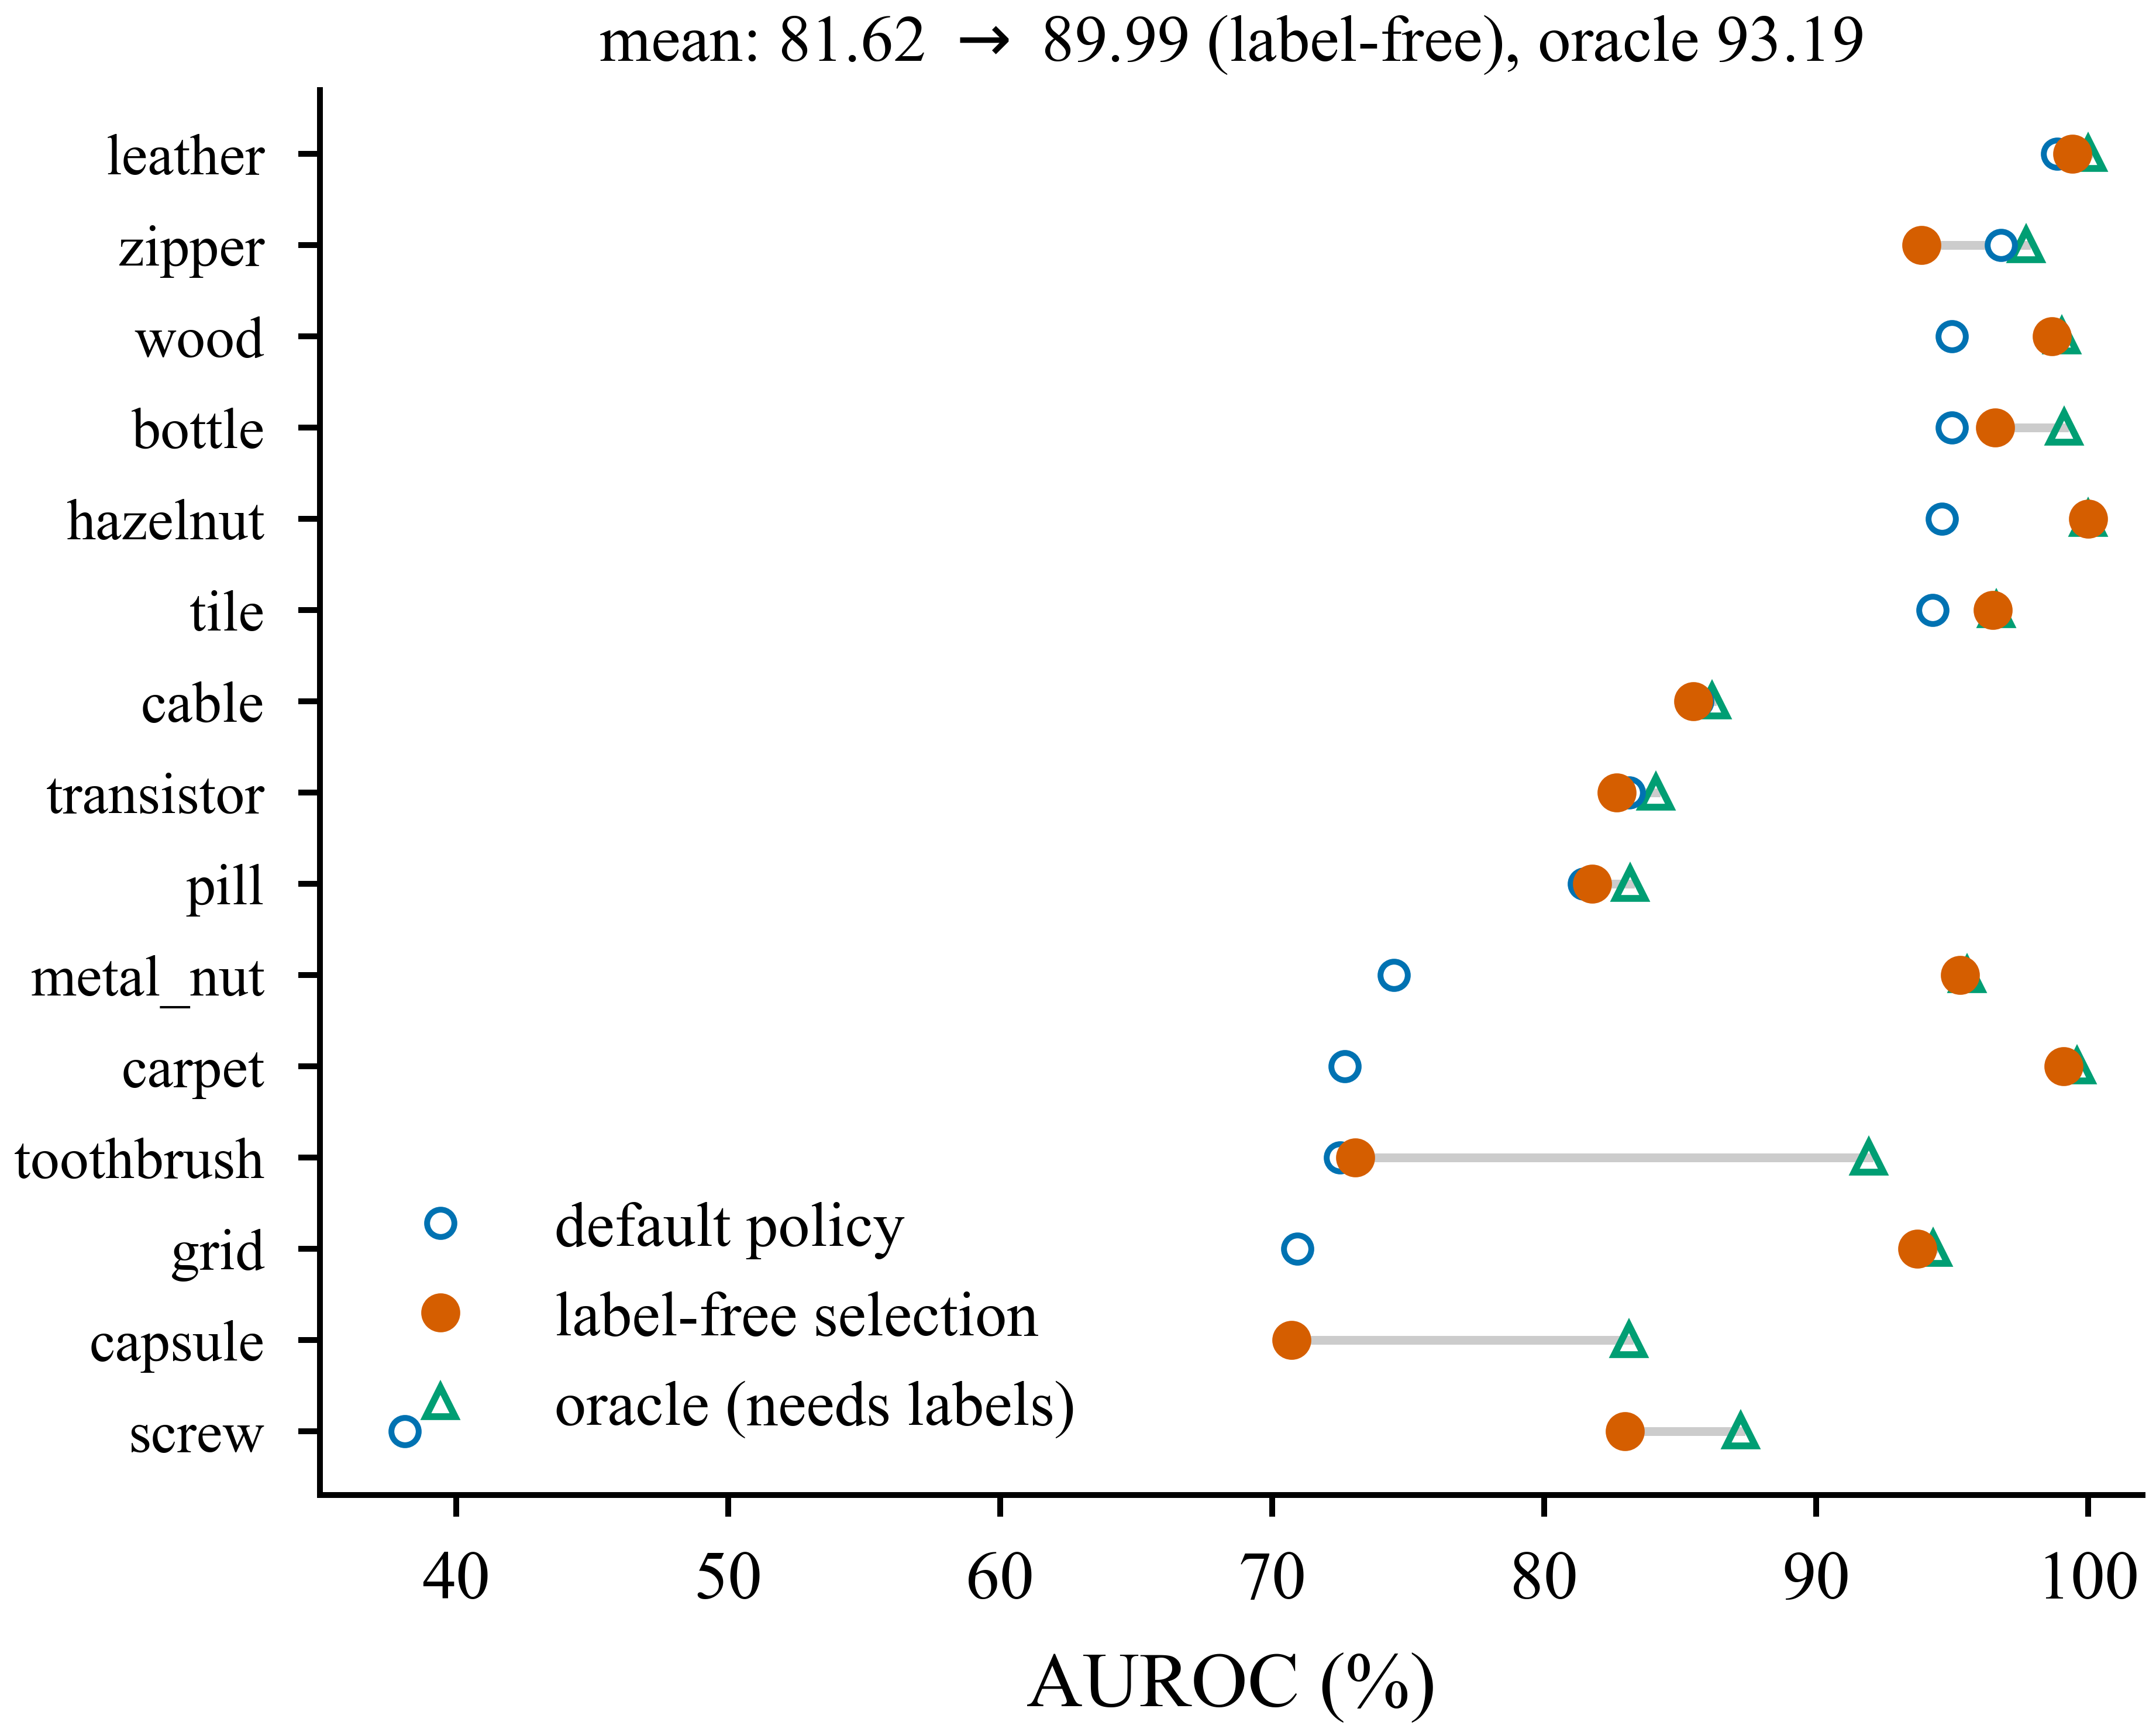
\includegraphics[width=\linewidth]{figures_v2/fig6_label_free_selection.png}
\caption{Label-free selection per category (seed 42). Hollow markers are the
published default policy, filled markers the policy chosen from synthetic
pseudo-anomalies without any anomaly label, and triangles the per-category oracle.
The label-free procedure recovers most of the available gap, and most of it on the
categories where the default policy fails badly (\texttt{screw}, \texttt{grid}).}
\label{fig:label_free}
\end{figure}

of the normal training images, with the remaining 30\% held out for selection
(the seed-42 default row is therefore $81.62\%$ rather than the $82.80\%$ of
Table~\ref{tab:fusion}, which uses the full training set). The gain is a
within-model comparison and is not inflated by the split; absolute numbers,
however, should be read with the split in mind.

\runinhead{Why the discriminative criterion works where the distributional one
fails.} The two criteria differ in what they ask of a clean image. The
distributional criterion asks that clean images look homogeneous, which top-$k$
pooling actively defeats. The discriminative criterion asks only that the policy
separate perturbed from clean --- the same question the detector is ultimately
asked at test time, posed on synthetic defects. It is a weaker and better-aimed
question, and it is answerable from normal data alone. Its own variance is the
open problem, not its direction.
